\documentclass[twoside]{book}

% Packages required by doxygen
\usepackage{fixltx2e}
\usepackage{calc}
\usepackage{doxygen}
\usepackage[export]{adjustbox} % also loads graphicx
\usepackage{graphicx}
\usepackage[utf8]{inputenc}
\usepackage{makeidx}
\usepackage{multicol}
\usepackage{multirow}
\PassOptionsToPackage{warn}{textcomp}
\usepackage{textcomp}
\usepackage[nointegrals]{wasysym}
\usepackage[table]{xcolor}

% Font selection
\usepackage[T1]{fontenc}
\usepackage[scaled=.90]{helvet}
\usepackage{courier}
\usepackage{amssymb}
\usepackage{sectsty}
\renewcommand{\familydefault}{\sfdefault}
\allsectionsfont{%
  \fontseries{bc}\selectfont%
  \color{darkgray}%
}
\renewcommand{\DoxyLabelFont}{%
  \fontseries{bc}\selectfont%
  \color{darkgray}%
}
\newcommand{\+}{\discretionary{\mbox{\scriptsize$\hookleftarrow$}}{}{}}

% Page & text layout
\usepackage{geometry}
\geometry{%
  a4paper,%
  top=2.5cm,%
  bottom=2.5cm,%
  left=2.5cm,%
  right=2.5cm%
}
\tolerance=750
\hfuzz=15pt
\hbadness=750
\setlength{\emergencystretch}{15pt}
\setlength{\parindent}{0cm}
\setlength{\parskip}{3ex plus 2ex minus 2ex}
\makeatletter
\renewcommand{\paragraph}{%
  \@startsection{paragraph}{4}{0ex}{-1.0ex}{1.0ex}{%
    \normalfont\normalsize\bfseries\SS@parafont%
  }%
}
\renewcommand{\subparagraph}{%
  \@startsection{subparagraph}{5}{0ex}{-1.0ex}{1.0ex}{%
    \normalfont\normalsize\bfseries\SS@subparafont%
  }%
}
\makeatother

% Headers & footers
\usepackage{fancyhdr}
\pagestyle{fancyplain}
\fancyhead[LE]{\fancyplain{}{\bfseries\thepage}}
\fancyhead[CE]{\fancyplain{}{}}
\fancyhead[RE]{\fancyplain{}{\bfseries\leftmark}}
\fancyhead[LO]{\fancyplain{}{\bfseries\rightmark}}
\fancyhead[CO]{\fancyplain{}{}}
\fancyhead[RO]{\fancyplain{}{\bfseries\thepage}}
\fancyfoot[LE]{\fancyplain{}{}}
\fancyfoot[CE]{\fancyplain{}{}}
\fancyfoot[RE]{\fancyplain{}{\bfseries\scriptsize Generated by Doxygen }}
\fancyfoot[LO]{\fancyplain{}{\bfseries\scriptsize Generated by Doxygen }}
\fancyfoot[CO]{\fancyplain{}{}}
\fancyfoot[RO]{\fancyplain{}{}}
\renewcommand{\footrulewidth}{0.4pt}
\renewcommand{\chaptermark}[1]{%
  \markboth{#1}{}%
}
\renewcommand{\sectionmark}[1]{%
  \markright{\thesection\ #1}%
}

% Indices & bibliography
\usepackage{natbib}
\usepackage[titles]{tocloft}
\setcounter{tocdepth}{3}
\setcounter{secnumdepth}{5}
\makeindex

% Hyperlinks (required, but should be loaded last)
\usepackage{ifpdf}
\ifpdf
  \usepackage[pdftex,pagebackref=true]{hyperref}
\else
  \usepackage[ps2pdf,pagebackref=true]{hyperref}
\fi
\hypersetup{%
  colorlinks=true,%
  linkcolor=blue,%
  citecolor=blue,%
  unicode%
}

% Custom commands
\newcommand{\clearemptydoublepage}{%
  \newpage{\pagestyle{empty}\cleardoublepage}%
}

\usepackage{caption}
\captionsetup{labelsep=space,justification=centering,font={bf},singlelinecheck=off,skip=4pt,position=top}

%===== C O N T E N T S =====

\begin{document}

% Titlepage & ToC
\hypersetup{pageanchor=false,
             bookmarksnumbered=true,
             pdfencoding=unicode
            }
\pagenumbering{alph}
\begin{titlepage}
\vspace*{7cm}
\begin{center}%
{\Large summerschool E\+S\+P32 }\\
\vspace*{1cm}
{\large Generated by Doxygen 1.8.13}\\
\end{center}
\end{titlepage}
\clearemptydoublepage
\pagenumbering{roman}
\tableofcontents
\clearemptydoublepage
\pagenumbering{arabic}
\hypersetup{pageanchor=true}

%--- Begin generated contents ---
\chapter{Namespace Index}
\section{Namespace List}
Here is a list of all namespaces with brief descriptions\+:\begin{DoxyCompactList}
\item\contentsline{section}{\hyperlink{namespace_ui}{Ui} }{\pageref{namespace_ui}}{}
\end{DoxyCompactList}

\chapter{Hierarchical Index}
\section{Class Hierarchy}
This inheritance list is sorted roughly, but not completely, alphabetically\+:\begin{DoxyCompactList}
\item \contentsline{section}{logger}{\pageref{classlogger}}{}
\item Q\+Dialog\begin{DoxyCompactList}
\item \contentsline{section}{C\+S\+Vread}{\pageref{class_c_s_vread}}{}
\item \contentsline{section}{Serial\+Port\+Settings}{\pageref{class_serial_port_settings}}{}
\item \contentsline{section}{wifisettings}{\pageref{classwifisettings}}{}
\end{DoxyCompactList}
\item Q\+Main\+Window\begin{DoxyCompactList}
\item \contentsline{section}{Main\+Window}{\pageref{class_main_window}}{}
\end{DoxyCompactList}
\item Q\+Object\begin{DoxyCompactList}
\item \contentsline{section}{E\+S\+P32data}{\pageref{class_e_s_p32data}}{}
\end{DoxyCompactList}
\item \contentsline{section}{E\+S\+P32data\+:\+:Wifi\+Settings}{\pageref{struct_e_s_p32data_1_1_wifi_settings}}{}
\end{DoxyCompactList}

\chapter{Class Index}
\section{Data Structures}
Here are the data structures with brief descriptions\+:\begin{DoxyCompactList}
\item\contentsline{section}{\hyperlink{structtimer__event__t}{timer\+\_\+event\+\_\+t} }{\pageref{structtimer__event__t}}{}
\end{DoxyCompactList}

\chapter{File Index}
\section{File List}
Here is a list of all files with brief descriptions\+:\begin{DoxyCompactList}
\item\contentsline{section}{C\+:/\+Users/\+Kuba/\+Documents/\+E\+S\+P32tool/\hyperlink{csvread_8cpp}{csvread.\+cpp} }{\pageref{csvread_8cpp}}{}
\item\contentsline{section}{C\+:/\+Users/\+Kuba/\+Documents/\+E\+S\+P32tool/\hyperlink{csvread_8h}{csvread.\+h} }{\pageref{csvread_8h}}{}
\item\contentsline{section}{C\+:/\+Users/\+Kuba/\+Documents/\+E\+S\+P32tool/\hyperlink{esp32data_8cpp}{esp32data.\+cpp} }{\pageref{esp32data_8cpp}}{}
\item\contentsline{section}{C\+:/\+Users/\+Kuba/\+Documents/\+E\+S\+P32tool/\hyperlink{esp32data_8h}{esp32data.\+h} }{\pageref{esp32data_8h}}{}
\item\contentsline{section}{C\+:/\+Users/\+Kuba/\+Documents/\+E\+S\+P32tool/\hyperlink{logger_8cpp}{logger.\+cpp} }{\pageref{logger_8cpp}}{}
\item\contentsline{section}{C\+:/\+Users/\+Kuba/\+Documents/\+E\+S\+P32tool/\hyperlink{logger_8h}{logger.\+h} }{\pageref{logger_8h}}{}
\item\contentsline{section}{C\+:/\+Users/\+Kuba/\+Documents/\+E\+S\+P32tool/\hyperlink{main_8cpp}{main.\+cpp} }{\pageref{main_8cpp}}{}
\item\contentsline{section}{C\+:/\+Users/\+Kuba/\+Documents/\+E\+S\+P32tool/\hyperlink{mainwindow_8cpp}{mainwindow.\+cpp} }{\pageref{mainwindow_8cpp}}{}
\item\contentsline{section}{C\+:/\+Users/\+Kuba/\+Documents/\+E\+S\+P32tool/\hyperlink{mainwindow_8h}{mainwindow.\+h} }{\pageref{mainwindow_8h}}{}
\item\contentsline{section}{C\+:/\+Users/\+Kuba/\+Documents/\+E\+S\+P32tool/\hyperlink{serialportsettings_8cpp}{serialportsettings.\+cpp} }{\pageref{serialportsettings_8cpp}}{}
\item\contentsline{section}{C\+:/\+Users/\+Kuba/\+Documents/\+E\+S\+P32tool/\hyperlink{serialportsettings_8h}{serialportsettings.\+h} }{\pageref{serialportsettings_8h}}{}
\item\contentsline{section}{C\+:/\+Users/\+Kuba/\+Documents/\+E\+S\+P32tool/\hyperlink{wifisettings_8cpp}{wifisettings.\+cpp} }{\pageref{wifisettings_8cpp}}{}
\item\contentsline{section}{C\+:/\+Users/\+Kuba/\+Documents/\+E\+S\+P32tool/\hyperlink{wifisettings_8h}{wifisettings.\+h} }{\pageref{wifisettings_8h}}{}
\end{DoxyCompactList}

\chapter{Namespace Documentation}
\hypertarget{namespace_ui}{}\section{Ui Namespace Reference}
\label{namespace_ui}\index{Ui@{Ui}}

\chapter{Class Documentation}
\hypertarget{class_c_s_vread}{}\section{C\+S\+Vread Class Reference}
\label{class_c_s_vread}\index{C\+S\+Vread@{C\+S\+Vread}}


{\ttfamily \#include $<$csvread.\+h$>$}

Inheritance diagram for C\+S\+Vread\+:\begin{figure}[H]
\begin{center}
\leavevmode
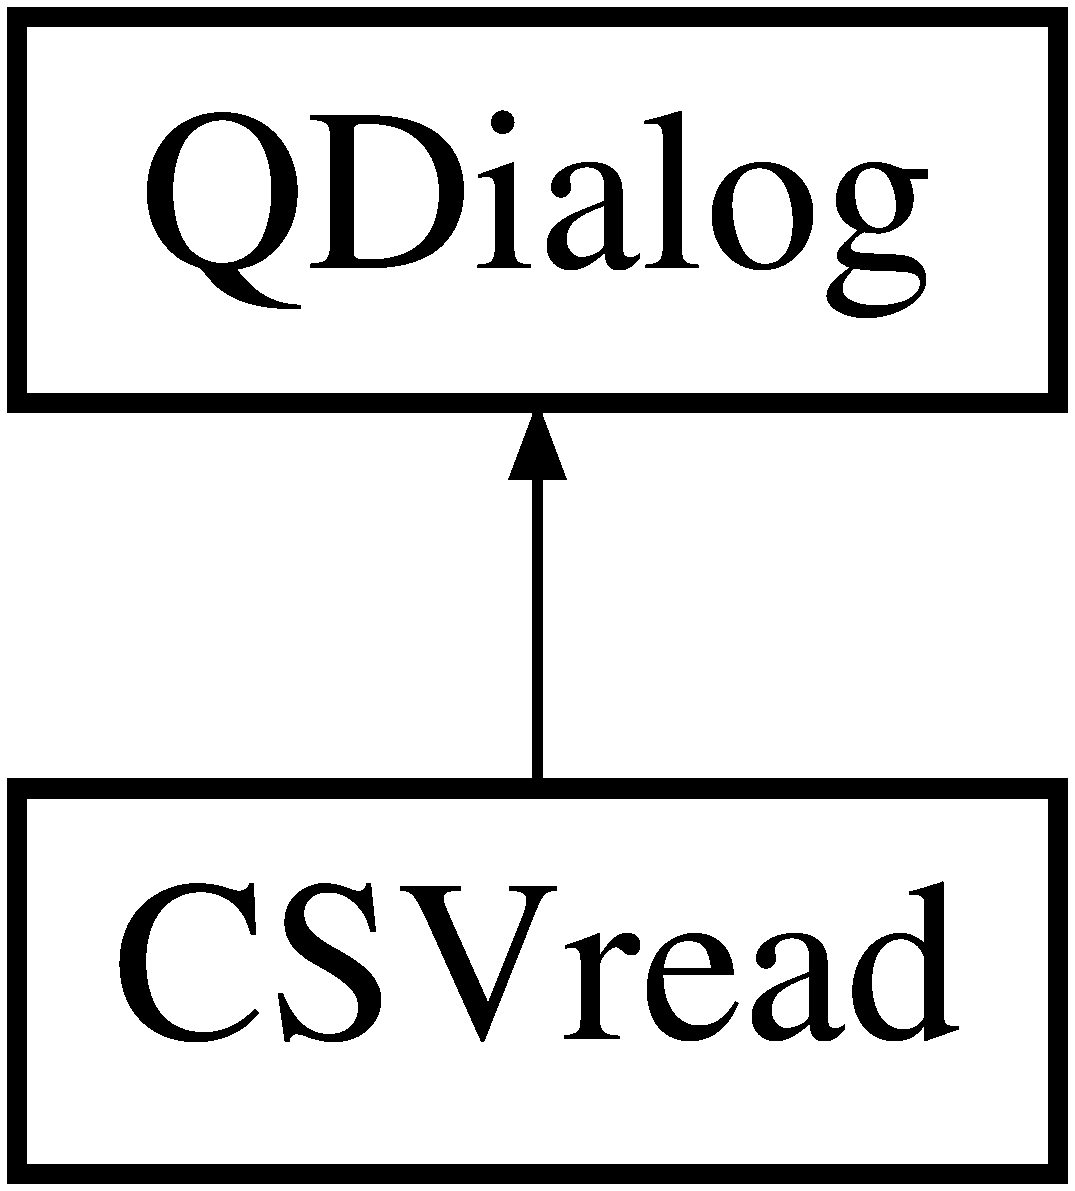
\includegraphics[height=2.000000cm]{class_c_s_vread}
\end{center}
\end{figure}
\subsection*{Public Member Functions}
\begin{DoxyCompactItemize}
\item 
\hyperlink{class_c_s_vread_a9677b85132c543c5a7eb4a2e4a3c95a0}{C\+S\+Vread} (Q\+Widget $\ast$parent=0)
\item 
bool \hyperlink{class_c_s_vread_a919b38bb6b737c7c9cbe5048e6e4b472}{initiate\+Window} ()
\begin{DoxyCompactList}\small\item\em initiate\+Window opens a window where we can select csv file to load and put it into table \end{DoxyCompactList}\item 
\hyperlink{class_c_s_vread_a8cac0f7ebeaed0c74581791229ab9b25}{$\sim$\+C\+S\+Vread} ()
\end{DoxyCompactItemize}


\subsection{Constructor \& Destructor Documentation}
\mbox{\Hypertarget{class_c_s_vread_a9677b85132c543c5a7eb4a2e4a3c95a0}\label{class_c_s_vread_a9677b85132c543c5a7eb4a2e4a3c95a0}} 
\index{C\+S\+Vread@{C\+S\+Vread}!C\+S\+Vread@{C\+S\+Vread}}
\index{C\+S\+Vread@{C\+S\+Vread}!C\+S\+Vread@{C\+S\+Vread}}
\subsubsection{\texorpdfstring{C\+S\+Vread()}{CSVread()}}
{\footnotesize\ttfamily C\+S\+Vread\+::\+C\+S\+Vread (\begin{DoxyParamCaption}\item[{Q\+Widget $\ast$}]{parent = {\ttfamily 0} }\end{DoxyParamCaption})\hspace{0.3cm}{\ttfamily [explicit]}}

\mbox{\Hypertarget{class_c_s_vread_a8cac0f7ebeaed0c74581791229ab9b25}\label{class_c_s_vread_a8cac0f7ebeaed0c74581791229ab9b25}} 
\index{C\+S\+Vread@{C\+S\+Vread}!````~C\+S\+Vread@{$\sim$\+C\+S\+Vread}}
\index{````~C\+S\+Vread@{$\sim$\+C\+S\+Vread}!C\+S\+Vread@{C\+S\+Vread}}
\subsubsection{\texorpdfstring{$\sim$\+C\+S\+Vread()}{~CSVread()}}
{\footnotesize\ttfamily C\+S\+Vread\+::$\sim$\+C\+S\+Vread (\begin{DoxyParamCaption}{ }\end{DoxyParamCaption})}



\subsection{Member Function Documentation}
\mbox{\Hypertarget{class_c_s_vread_a919b38bb6b737c7c9cbe5048e6e4b472}\label{class_c_s_vread_a919b38bb6b737c7c9cbe5048e6e4b472}} 
\index{C\+S\+Vread@{C\+S\+Vread}!initiate\+Window@{initiate\+Window}}
\index{initiate\+Window@{initiate\+Window}!C\+S\+Vread@{C\+S\+Vread}}
\subsubsection{\texorpdfstring{initiate\+Window()}{initiateWindow()}}
{\footnotesize\ttfamily bool C\+S\+Vread\+::initiate\+Window (\begin{DoxyParamCaption}{ }\end{DoxyParamCaption})}



initiate\+Window opens a window where we can select csv file to load and put it into table 

\begin{DoxyReturn}{Returns}
T\+R\+UE = successful opened file, F\+A\+L\+SE = didn\textquotesingle{}t manage to open file 
\end{DoxyReturn}


The documentation for this class was generated from the following files\+:\begin{DoxyCompactItemize}
\item 
C\+:/\+Users/\+Kuba/\+Documents/\+E\+S\+P32tool/\hyperlink{csvread_8h}{csvread.\+h}\item 
C\+:/\+Users/\+Kuba/\+Documents/\+E\+S\+P32tool/\hyperlink{csvread_8cpp}{csvread.\+cpp}\end{DoxyCompactItemize}

\hypertarget{class_e_s_p32data}{}\section{E\+S\+P32data Class Reference}
\label{class_e_s_p32data}\index{E\+S\+P32data@{E\+S\+P32data}}


{\ttfamily \#include $<$esp32data.\+h$>$}

Inheritance diagram for E\+S\+P32data\+:\begin{figure}[H]
\begin{center}
\leavevmode
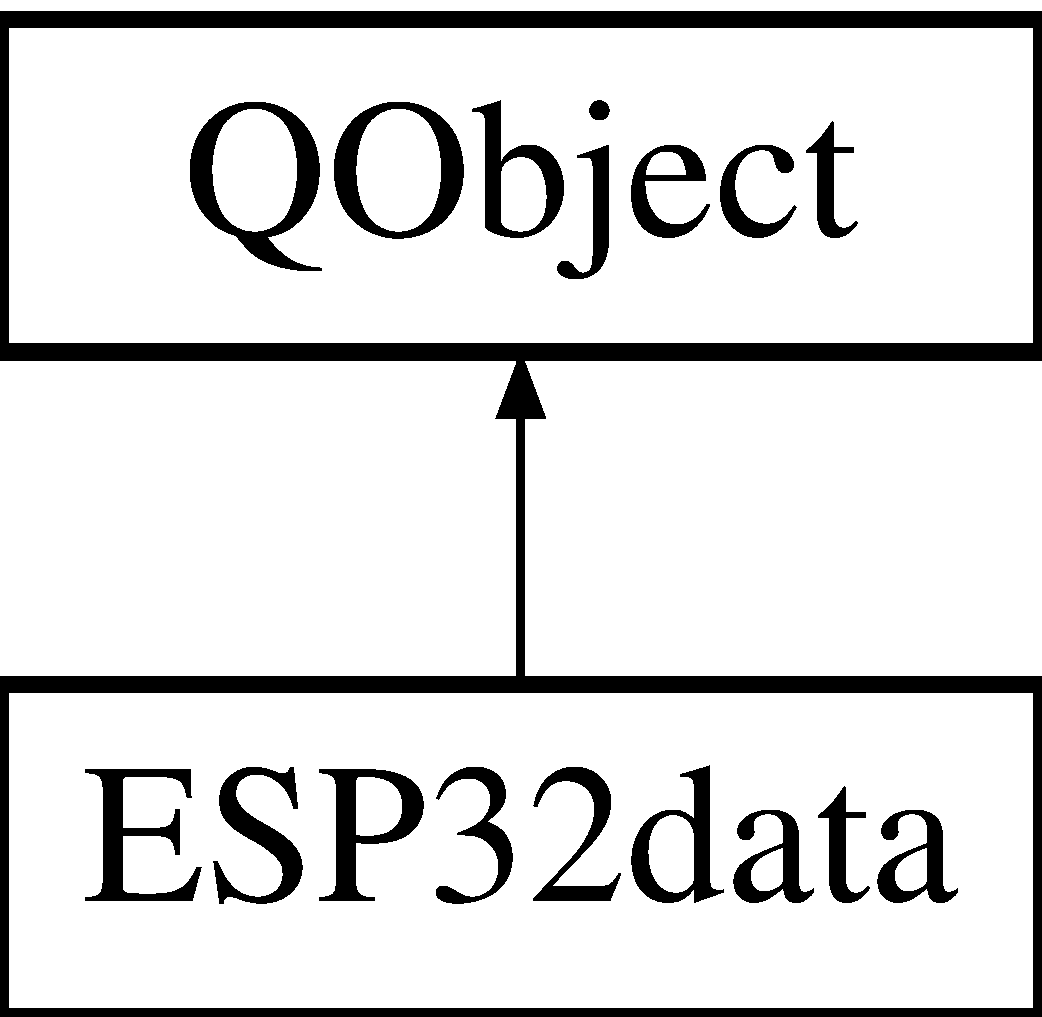
\includegraphics[height=2.000000cm]{class_e_s_p32data}
\end{center}
\end{figure}
\subsection*{Classes}
\begin{DoxyCompactItemize}
\item 
struct \hyperlink{struct_e_s_p32data_1_1_wifi_settings}{Wifi\+Settings}
\end{DoxyCompactItemize}
\subsection*{Public Slots}
\begin{DoxyCompactItemize}
\item 
void \hyperlink{class_e_s_p32data_ad2205a1545fbea3bff74848dc43c4684}{set\+Gpios} (int pin1, int pin2)
\begin{DoxyCompactList}\small\item\em set\+Gpios set pins levels and send frame \end{DoxyCompactList}\item 
void \hyperlink{class_e_s_p32data_aa2716175de492c5de8bb48333eafd9a2}{set\+Frequency\+Adc} (double freq)
\begin{DoxyCompactList}\small\item\em set\+Frequency\+Adc and send frame \end{DoxyCompactList}\item 
void \hyperlink{class_e_s_p32data_a38e856c9f7c5c986fee548ff2e9980a3}{timer\+Event} (Q\+Timer\+Event $\ast$ev)
\begin{DoxyCompactList}\small\item\em timer\+Event timer which contains getting data from E\+S\+P32 \end{DoxyCompactList}\item 
void \hyperlink{class_e_s_p32data_acce7a248a76cc084a78d58aa0b8d18ae}{write\+Data} (Q\+Byte\+Array data)
\begin{DoxyCompactList}\small\item\em write\+Data send data on U\+A\+RT \end{DoxyCompactList}\item 
void \hyperlink{class_e_s_p32data_a50a3a6adc1a17b1d59e57c1ead7b369d}{call\+For\+Data} ()
\begin{DoxyCompactList}\small\item\em call\+For\+Data sends a frame and then E\+S\+P32 answers adcs values in frame \end{DoxyCompactList}\item 
Q\+Byte\+Array \hyperlink{class_e_s_p32data_aacb815132c382980c4d850f099e26ea6}{read\+Data} ()
\begin{DoxyCompactList}\small\item\em read\+Data read data from uart \end{DoxyCompactList}\item 
void \hyperlink{class_e_s_p32data_ab474f90be7784fdc763e78d6bb741c91}{read\+Pending\+Datagrams} ()
\begin{DoxyCompactList}\small\item\em read\+Pending\+Datagrams receive datagrams in U\+DP \end{DoxyCompactList}\end{DoxyCompactItemize}
\subsection*{Signals}
\begin{DoxyCompactItemize}
\item 
void \hyperlink{class_e_s_p32data_ade36e3d9b929614a79d1a24491c18185}{new\+Data\+Adc} (int, int)
\begin{DoxyCompactList}\small\item\em new\+Data\+Adc we get data and emit a signal-\/ we send adc1 and adc2 values in arguments(\+Q\+T automaticy get it it when we connect with slot) after connecting data go to slot and we can process this data in the slot \end{DoxyCompactList}\end{DoxyCompactItemize}
\subsection*{Public Member Functions}
\begin{DoxyCompactItemize}
\item 
\hyperlink{class_e_s_p32data_a23df6c4c56c578b115900d767280ed78}{E\+S\+P32data} (Q\+Object $\ast$parent=0)
\begin{DoxyCompactList}\small\item\em \hyperlink{class_e_s_p32data}{E\+S\+P32data} class is used to communication with E\+SP module, it doesn\textquotesingle{}t create any windows,it just class for communication. \end{DoxyCompactList}\item 
void \hyperlink{class_e_s_p32data_a74a82e4ce7f99e01b1c9e1f6e3cd6333}{close\+Port} ()
\begin{DoxyCompactList}\small\item\em close\+Port closing uart communication port \end{DoxyCompactList}\item 
void \hyperlink{class_e_s_p32data_a6681c1880617d85c2dfe2dac976aa021}{set\+Port} (Q\+String Name\+Port)
\begin{DoxyCompactList}\small\item\em set\+Port selects port in computer where E\+S\+P32 is connected, for example C\+O\+M3 \end{DoxyCompactList}\item 
Q\+String \hyperlink{class_e_s_p32data_a7f451228e41241eb51347d6453f30590}{get\+Port} ()
\item 
void \hyperlink{class_e_s_p32data_a48f03ba841041fd88b8c60659ef36064}{init\+Socket} ()
\begin{DoxyCompactList}\small\item\em init\+Socket opens a socket on a computer, in summerschool computer was a server and E\+SP was a client \end{DoxyCompactList}\item 
void \hyperlink{class_e_s_p32data_ac4d3568c735d68b89cc5c7d59ccce8e7}{set\+Wifi\+Settings} ()
\begin{DoxyCompactList}\small\item\em set\+Wifi\+Settings it loads values from window and sends it to E\+S\+P32 in frame, T\+O\+DO\+: \hyperlink{struct_e_s_p32data_1_1_wifi_settings}{Wifi\+Settings} struct is public-\/ change it \end{DoxyCompactList}\item 
\hyperlink{class_e_s_p32data_ae250e8a91371316a8104e65328cef89d}{$\sim$\+E\+S\+P32data} ()
\end{DoxyCompactItemize}
\subsection*{Public Attributes}
\begin{DoxyCompactItemize}
\item 
\hyperlink{struct_e_s_p32data_1_1_wifi_settings}{Wifi\+Settings} \hyperlink{class_e_s_p32data_af22a2683c01fae73c97eb0e03884675b}{wificonnection}
\end{DoxyCompactItemize}


\subsection{Constructor \& Destructor Documentation}
\mbox{\Hypertarget{class_e_s_p32data_a23df6c4c56c578b115900d767280ed78}\label{class_e_s_p32data_a23df6c4c56c578b115900d767280ed78}} 
\index{E\+S\+P32data@{E\+S\+P32data}!E\+S\+P32data@{E\+S\+P32data}}
\index{E\+S\+P32data@{E\+S\+P32data}!E\+S\+P32data@{E\+S\+P32data}}
\subsubsection{\texorpdfstring{E\+S\+P32data()}{ESP32data()}}
{\footnotesize\ttfamily E\+S\+P32data\+::\+E\+S\+P32data (\begin{DoxyParamCaption}\item[{Q\+Object $\ast$}]{parent = {\ttfamily 0} }\end{DoxyParamCaption})\hspace{0.3cm}{\ttfamily [explicit]}}



\hyperlink{class_e_s_p32data}{E\+S\+P32data} class is used to communication with E\+SP module, it doesn\textquotesingle{}t create any windows,it just class for communication. 

\mbox{\Hypertarget{class_e_s_p32data_ae250e8a91371316a8104e65328cef89d}\label{class_e_s_p32data_ae250e8a91371316a8104e65328cef89d}} 
\index{E\+S\+P32data@{E\+S\+P32data}!````~E\+S\+P32data@{$\sim$\+E\+S\+P32data}}
\index{````~E\+S\+P32data@{$\sim$\+E\+S\+P32data}!E\+S\+P32data@{E\+S\+P32data}}
\subsubsection{\texorpdfstring{$\sim$\+E\+S\+P32data()}{~ESP32data()}}
{\footnotesize\ttfamily E\+S\+P32data\+::$\sim$\+E\+S\+P32data (\begin{DoxyParamCaption}{ }\end{DoxyParamCaption})}



\subsection{Member Function Documentation}
\mbox{\Hypertarget{class_e_s_p32data_a50a3a6adc1a17b1d59e57c1ead7b369d}\label{class_e_s_p32data_a50a3a6adc1a17b1d59e57c1ead7b369d}} 
\index{E\+S\+P32data@{E\+S\+P32data}!call\+For\+Data@{call\+For\+Data}}
\index{call\+For\+Data@{call\+For\+Data}!E\+S\+P32data@{E\+S\+P32data}}
\subsubsection{\texorpdfstring{call\+For\+Data}{callForData}}
{\footnotesize\ttfamily void E\+S\+P32data\+::call\+For\+Data (\begin{DoxyParamCaption}{ }\end{DoxyParamCaption})\hspace{0.3cm}{\ttfamily [slot]}}



call\+For\+Data sends a frame and then E\+S\+P32 answers adcs values in frame 

\mbox{\Hypertarget{class_e_s_p32data_a74a82e4ce7f99e01b1c9e1f6e3cd6333}\label{class_e_s_p32data_a74a82e4ce7f99e01b1c9e1f6e3cd6333}} 
\index{E\+S\+P32data@{E\+S\+P32data}!close\+Port@{close\+Port}}
\index{close\+Port@{close\+Port}!E\+S\+P32data@{E\+S\+P32data}}
\subsubsection{\texorpdfstring{close\+Port()}{closePort()}}
{\footnotesize\ttfamily void E\+S\+P32data\+::close\+Port (\begin{DoxyParamCaption}{ }\end{DoxyParamCaption})}



close\+Port closing uart communication port 

\mbox{\Hypertarget{class_e_s_p32data_a7f451228e41241eb51347d6453f30590}\label{class_e_s_p32data_a7f451228e41241eb51347d6453f30590}} 
\index{E\+S\+P32data@{E\+S\+P32data}!get\+Port@{get\+Port}}
\index{get\+Port@{get\+Port}!E\+S\+P32data@{E\+S\+P32data}}
\subsubsection{\texorpdfstring{get\+Port()}{getPort()}}
{\footnotesize\ttfamily Q\+String E\+S\+P32data\+::get\+Port (\begin{DoxyParamCaption}{ }\end{DoxyParamCaption})}

\mbox{\Hypertarget{class_e_s_p32data_a48f03ba841041fd88b8c60659ef36064}\label{class_e_s_p32data_a48f03ba841041fd88b8c60659ef36064}} 
\index{E\+S\+P32data@{E\+S\+P32data}!init\+Socket@{init\+Socket}}
\index{init\+Socket@{init\+Socket}!E\+S\+P32data@{E\+S\+P32data}}
\subsubsection{\texorpdfstring{init\+Socket()}{initSocket()}}
{\footnotesize\ttfamily void E\+S\+P32data\+::init\+Socket (\begin{DoxyParamCaption}{ }\end{DoxyParamCaption})}



init\+Socket opens a socket on a computer, in summerschool computer was a server and E\+SP was a client 

\mbox{\Hypertarget{class_e_s_p32data_ade36e3d9b929614a79d1a24491c18185}\label{class_e_s_p32data_ade36e3d9b929614a79d1a24491c18185}} 
\index{E\+S\+P32data@{E\+S\+P32data}!new\+Data\+Adc@{new\+Data\+Adc}}
\index{new\+Data\+Adc@{new\+Data\+Adc}!E\+S\+P32data@{E\+S\+P32data}}
\subsubsection{\texorpdfstring{new\+Data\+Adc}{newDataAdc}}
{\footnotesize\ttfamily void E\+S\+P32data\+::new\+Data\+Adc (\begin{DoxyParamCaption}\item[{int}]{,  }\item[{int}]{ }\end{DoxyParamCaption})\hspace{0.3cm}{\ttfamily [signal]}}



new\+Data\+Adc we get data and emit a signal-\/ we send adc1 and adc2 values in arguments(\+Q\+T automaticy get it it when we connect with slot) after connecting data go to slot and we can process this data in the slot 

\mbox{\Hypertarget{class_e_s_p32data_aacb815132c382980c4d850f099e26ea6}\label{class_e_s_p32data_aacb815132c382980c4d850f099e26ea6}} 
\index{E\+S\+P32data@{E\+S\+P32data}!read\+Data@{read\+Data}}
\index{read\+Data@{read\+Data}!E\+S\+P32data@{E\+S\+P32data}}
\subsubsection{\texorpdfstring{read\+Data}{readData}}
{\footnotesize\ttfamily Q\+Byte\+Array E\+S\+P32data\+::read\+Data (\begin{DoxyParamCaption}{ }\end{DoxyParamCaption})\hspace{0.3cm}{\ttfamily [slot]}}



read\+Data read data from uart 

\begin{DoxyReturn}{Returns}

\end{DoxyReturn}
\mbox{\Hypertarget{class_e_s_p32data_ab474f90be7784fdc763e78d6bb741c91}\label{class_e_s_p32data_ab474f90be7784fdc763e78d6bb741c91}} 
\index{E\+S\+P32data@{E\+S\+P32data}!read\+Pending\+Datagrams@{read\+Pending\+Datagrams}}
\index{read\+Pending\+Datagrams@{read\+Pending\+Datagrams}!E\+S\+P32data@{E\+S\+P32data}}
\subsubsection{\texorpdfstring{read\+Pending\+Datagrams}{readPendingDatagrams}}
{\footnotesize\ttfamily void E\+S\+P32data\+::read\+Pending\+Datagrams (\begin{DoxyParamCaption}{ }\end{DoxyParamCaption})\hspace{0.3cm}{\ttfamily [slot]}}



read\+Pending\+Datagrams receive datagrams in U\+DP 

\mbox{\Hypertarget{class_e_s_p32data_aa2716175de492c5de8bb48333eafd9a2}\label{class_e_s_p32data_aa2716175de492c5de8bb48333eafd9a2}} 
\index{E\+S\+P32data@{E\+S\+P32data}!set\+Frequency\+Adc@{set\+Frequency\+Adc}}
\index{set\+Frequency\+Adc@{set\+Frequency\+Adc}!E\+S\+P32data@{E\+S\+P32data}}
\subsubsection{\texorpdfstring{set\+Frequency\+Adc}{setFrequencyAdc}}
{\footnotesize\ttfamily void E\+S\+P32data\+::set\+Frequency\+Adc (\begin{DoxyParamCaption}\item[{double}]{freq }\end{DoxyParamCaption})\hspace{0.3cm}{\ttfamily [slot]}}



set\+Frequency\+Adc and send frame 


\begin{DoxyParams}{Parameters}
{\em freq} & \\
\hline
\end{DoxyParams}
\mbox{\Hypertarget{class_e_s_p32data_ad2205a1545fbea3bff74848dc43c4684}\label{class_e_s_p32data_ad2205a1545fbea3bff74848dc43c4684}} 
\index{E\+S\+P32data@{E\+S\+P32data}!set\+Gpios@{set\+Gpios}}
\index{set\+Gpios@{set\+Gpios}!E\+S\+P32data@{E\+S\+P32data}}
\subsubsection{\texorpdfstring{set\+Gpios}{setGpios}}
{\footnotesize\ttfamily void E\+S\+P32data\+::set\+Gpios (\begin{DoxyParamCaption}\item[{int}]{pin1,  }\item[{int}]{pin2 }\end{DoxyParamCaption})\hspace{0.3cm}{\ttfamily [slot]}}



set\+Gpios set pins levels and send frame 


\begin{DoxyParams}{Parameters}
{\em pin1} & level \\
\hline
{\em pin2} & level \\
\hline
\end{DoxyParams}
\mbox{\Hypertarget{class_e_s_p32data_a6681c1880617d85c2dfe2dac976aa021}\label{class_e_s_p32data_a6681c1880617d85c2dfe2dac976aa021}} 
\index{E\+S\+P32data@{E\+S\+P32data}!set\+Port@{set\+Port}}
\index{set\+Port@{set\+Port}!E\+S\+P32data@{E\+S\+P32data}}
\subsubsection{\texorpdfstring{set\+Port()}{setPort()}}
{\footnotesize\ttfamily void E\+S\+P32data\+::set\+Port (\begin{DoxyParamCaption}\item[{Q\+String}]{Name\+Port }\end{DoxyParamCaption})}



set\+Port selects port in computer where E\+S\+P32 is connected, for example C\+O\+M3 


\begin{DoxyParams}{Parameters}
{\em Name\+Port} & port, example C\+O\+M3 \\
\hline
\end{DoxyParams}
\mbox{\Hypertarget{class_e_s_p32data_ac4d3568c735d68b89cc5c7d59ccce8e7}\label{class_e_s_p32data_ac4d3568c735d68b89cc5c7d59ccce8e7}} 
\index{E\+S\+P32data@{E\+S\+P32data}!set\+Wifi\+Settings@{set\+Wifi\+Settings}}
\index{set\+Wifi\+Settings@{set\+Wifi\+Settings}!E\+S\+P32data@{E\+S\+P32data}}
\subsubsection{\texorpdfstring{set\+Wifi\+Settings()}{setWifiSettings()}}
{\footnotesize\ttfamily void E\+S\+P32data\+::set\+Wifi\+Settings (\begin{DoxyParamCaption}{ }\end{DoxyParamCaption})}



set\+Wifi\+Settings it loads values from window and sends it to E\+S\+P32 in frame, T\+O\+DO\+: \hyperlink{struct_e_s_p32data_1_1_wifi_settings}{Wifi\+Settings} struct is public-\/ change it 

\mbox{\Hypertarget{class_e_s_p32data_a38e856c9f7c5c986fee548ff2e9980a3}\label{class_e_s_p32data_a38e856c9f7c5c986fee548ff2e9980a3}} 
\index{E\+S\+P32data@{E\+S\+P32data}!timer\+Event@{timer\+Event}}
\index{timer\+Event@{timer\+Event}!E\+S\+P32data@{E\+S\+P32data}}
\subsubsection{\texorpdfstring{timer\+Event}{timerEvent}}
{\footnotesize\ttfamily void E\+S\+P32data\+::timer\+Event (\begin{DoxyParamCaption}\item[{Q\+Timer\+Event $\ast$}]{ev }\end{DoxyParamCaption})\hspace{0.3cm}{\ttfamily [slot]}}



timer\+Event timer which contains getting data from E\+S\+P32 


\begin{DoxyParams}{Parameters}
{\em ev} & \\
\hline
\end{DoxyParams}
\mbox{\Hypertarget{class_e_s_p32data_acce7a248a76cc084a78d58aa0b8d18ae}\label{class_e_s_p32data_acce7a248a76cc084a78d58aa0b8d18ae}} 
\index{E\+S\+P32data@{E\+S\+P32data}!write\+Data@{write\+Data}}
\index{write\+Data@{write\+Data}!E\+S\+P32data@{E\+S\+P32data}}
\subsubsection{\texorpdfstring{write\+Data}{writeData}}
{\footnotesize\ttfamily void E\+S\+P32data\+::write\+Data (\begin{DoxyParamCaption}\item[{Q\+Byte\+Array}]{data }\end{DoxyParamCaption})\hspace{0.3cm}{\ttfamily [slot]}}



write\+Data send data on U\+A\+RT 


\begin{DoxyParams}{Parameters}
{\em data} & Q\+Byte\+Array data \\
\hline
\end{DoxyParams}


\subsection{Member Data Documentation}
\mbox{\Hypertarget{class_e_s_p32data_af22a2683c01fae73c97eb0e03884675b}\label{class_e_s_p32data_af22a2683c01fae73c97eb0e03884675b}} 
\index{E\+S\+P32data@{E\+S\+P32data}!wificonnection@{wificonnection}}
\index{wificonnection@{wificonnection}!E\+S\+P32data@{E\+S\+P32data}}
\subsubsection{\texorpdfstring{wificonnection}{wificonnection}}
{\footnotesize\ttfamily \hyperlink{struct_e_s_p32data_1_1_wifi_settings}{Wifi\+Settings} E\+S\+P32data\+::wificonnection}

struct object which contais wifi settings 

The documentation for this class was generated from the following files\+:\begin{DoxyCompactItemize}
\item 
C\+:/\+Users/\+Kuba/\+Documents/\+E\+S\+P32tool/\hyperlink{esp32data_8h}{esp32data.\+h}\item 
C\+:/\+Users/\+Kuba/\+Documents/\+E\+S\+P32tool/\hyperlink{esp32data_8cpp}{esp32data.\+cpp}\end{DoxyCompactItemize}

\hypertarget{classlogger}{}\section{logger Class Reference}
\label{classlogger}\index{logger@{logger}}


{\ttfamily \#include $<$logger.\+h$>$}

\subsection*{Public Slots}
\begin{DoxyCompactItemize}
\item 
void \hyperlink{classlogger_a6061365f51872f2f269568a8243dc284}{stop\+Saving} ()
\begin{DoxyCompactList}\small\item\em stop\+Saving sets flag that file is closed and close port \end{DoxyCompactList}\item 
void \hyperlink{classlogger_abfe4ff2446577ad695e9fed3fb3aec52}{log} (Q\+Vector$<$ int $>$ data)
\begin{DoxyCompactList}\small\item\em log logger to file time, adc1, adc2 \end{DoxyCompactList}\end{DoxyCompactItemize}
\subsection*{Public Member Functions}
\begin{DoxyCompactItemize}
\item 
\hyperlink{classlogger_a4f753a510e00c892b38e95c2284363a6}{logger} ()
\begin{DoxyCompactList}\small\item\em class used to save files \end{DoxyCompactList}\item 
void \hyperlink{classlogger_aa50d85f779b5f28f67dab8ab6a215ad8}{Open\+File} (Q\+String Save\+File\+Name)
\begin{DoxyCompactList}\small\item\em Open\+File. \end{DoxyCompactList}\item 
bool \hyperlink{classlogger_a1e070c45351986c87fe9c697b149de8d}{get\+Saving\+To\+File\+Flag} () const
\begin{DoxyCompactList}\small\item\em get\+Saving\+To\+File\+Flag \end{DoxyCompactList}\item 
\hyperlink{classlogger_aadd537feeeb16186f6aeb4ca0267a8d7}{$\sim$logger} ()
\end{DoxyCompactItemize}


\subsection{Constructor \& Destructor Documentation}
\mbox{\Hypertarget{classlogger_a4f753a510e00c892b38e95c2284363a6}\label{classlogger_a4f753a510e00c892b38e95c2284363a6}} 
\index{logger@{logger}!logger@{logger}}
\index{logger@{logger}!logger@{logger}}
\subsubsection{\texorpdfstring{logger()}{logger()}}
{\footnotesize\ttfamily logger\+::logger (\begin{DoxyParamCaption}{ }\end{DoxyParamCaption})}



class used to save files 

\mbox{\Hypertarget{classlogger_aadd537feeeb16186f6aeb4ca0267a8d7}\label{classlogger_aadd537feeeb16186f6aeb4ca0267a8d7}} 
\index{logger@{logger}!````~logger@{$\sim$logger}}
\index{````~logger@{$\sim$logger}!logger@{logger}}
\subsubsection{\texorpdfstring{$\sim$logger()}{~logger()}}
{\footnotesize\ttfamily logger\+::$\sim$logger (\begin{DoxyParamCaption}{ }\end{DoxyParamCaption})}



\subsection{Member Function Documentation}
\mbox{\Hypertarget{classlogger_a1e070c45351986c87fe9c697b149de8d}\label{classlogger_a1e070c45351986c87fe9c697b149de8d}} 
\index{logger@{logger}!get\+Saving\+To\+File\+Flag@{get\+Saving\+To\+File\+Flag}}
\index{get\+Saving\+To\+File\+Flag@{get\+Saving\+To\+File\+Flag}!logger@{logger}}
\subsubsection{\texorpdfstring{get\+Saving\+To\+File\+Flag()}{getSavingToFileFlag()}}
{\footnotesize\ttfamily bool logger\+::get\+Saving\+To\+File\+Flag (\begin{DoxyParamCaption}{ }\end{DoxyParamCaption}) const}



get\+Saving\+To\+File\+Flag 

\begin{DoxyReturn}{Returns}
true if file opened false if not opened 
\end{DoxyReturn}
\mbox{\Hypertarget{classlogger_abfe4ff2446577ad695e9fed3fb3aec52}\label{classlogger_abfe4ff2446577ad695e9fed3fb3aec52}} 
\index{logger@{logger}!log@{log}}
\index{log@{log}!logger@{logger}}
\subsubsection{\texorpdfstring{log}{log}}
{\footnotesize\ttfamily void logger\+::log (\begin{DoxyParamCaption}\item[{Q\+Vector$<$ int $>$}]{data }\end{DoxyParamCaption})\hspace{0.3cm}{\ttfamily [slot]}}



log logger to file time, adc1, adc2 


\begin{DoxyParams}{Parameters}
{\em data} & is vector with adc1 and adc2 data \\
\hline
\end{DoxyParams}
\mbox{\Hypertarget{classlogger_aa50d85f779b5f28f67dab8ab6a215ad8}\label{classlogger_aa50d85f779b5f28f67dab8ab6a215ad8}} 
\index{logger@{logger}!Open\+File@{Open\+File}}
\index{Open\+File@{Open\+File}!logger@{logger}}
\subsubsection{\texorpdfstring{Open\+File()}{OpenFile()}}
{\footnotesize\ttfamily void logger\+::\+Open\+File (\begin{DoxyParamCaption}\item[{Q\+String}]{Save\+File\+Name }\end{DoxyParamCaption})}



Open\+File. 


\begin{DoxyParams}{Parameters}
{\em Save\+File\+Name} & file which we use to save data \\
\hline
\end{DoxyParams}
\mbox{\Hypertarget{classlogger_a6061365f51872f2f269568a8243dc284}\label{classlogger_a6061365f51872f2f269568a8243dc284}} 
\index{logger@{logger}!stop\+Saving@{stop\+Saving}}
\index{stop\+Saving@{stop\+Saving}!logger@{logger}}
\subsubsection{\texorpdfstring{stop\+Saving}{stopSaving}}
{\footnotesize\ttfamily void logger\+::stop\+Saving (\begin{DoxyParamCaption}{ }\end{DoxyParamCaption})\hspace{0.3cm}{\ttfamily [slot]}}



stop\+Saving sets flag that file is closed and close port 



The documentation for this class was generated from the following files\+:\begin{DoxyCompactItemize}
\item 
C\+:/\+Users/\+Kuba/\+Documents/\+E\+S\+P32tool/\hyperlink{logger_8h}{logger.\+h}\item 
C\+:/\+Users/\+Kuba/\+Documents/\+E\+S\+P32tool/\hyperlink{logger_8cpp}{logger.\+cpp}\end{DoxyCompactItemize}

\hypertarget{class_main_window}{}\section{Main\+Window Class Reference}
\label{class_main_window}\index{Main\+Window@{Main\+Window}}


{\ttfamily \#include $<$mainwindow.\+h$>$}

Inheritance diagram for Main\+Window\+:\begin{figure}[H]
\begin{center}
\leavevmode
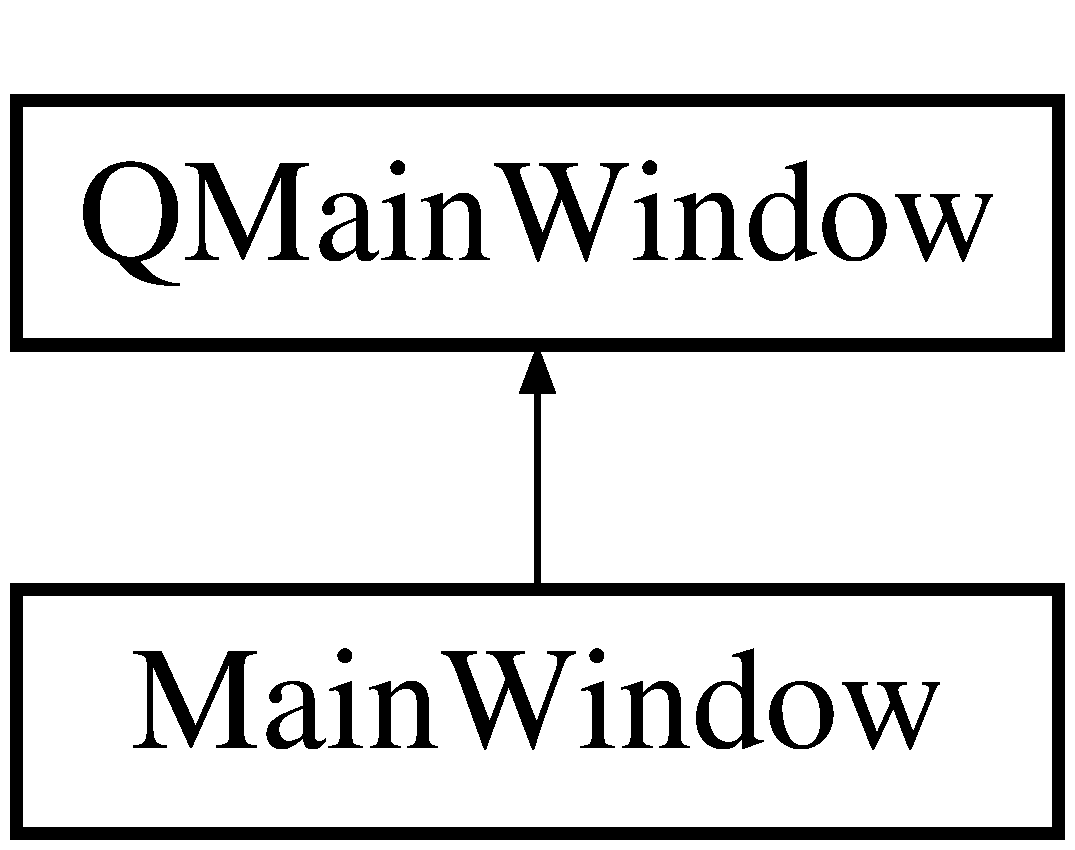
\includegraphics[height=2.000000cm]{class_main_window}
\end{center}
\end{figure}
\subsection*{Public Slots}
\begin{DoxyCompactItemize}
\item 
void \hyperlink{class_main_window_a0f0b8e878849a65e6c5b2405fe22f26e}{pokaz\+Komunikacja} (bool state)
\item 
void \hyperlink{class_main_window_a84238e487942aac887ca4702844ed26e}{pokaz\+Okno\+Wi\+Fi} (bool state)
\item 
void \hyperlink{class_main_window_ab12446607d3535de4c195ce03d2c62c1}{new\+Adc\+Data} (int adc1, int adc2)
\begin{DoxyCompactList}\small\item\em new\+Adc\+Data slot to receive data from emited signal, process adc values \end{DoxyCompactList}\item 
void \hyperlink{class_main_window_a02844dac36eef12a555efacba15722e3}{saving\+Clicked} (bool state)
\item 
void \hyperlink{class_main_window_a67bd4592c9f76e24a3e2398a6d362c5d}{pokaz\+C\+S\+Vreader} ()
\end{DoxyCompactItemize}
\subsection*{Public Member Functions}
\begin{DoxyCompactItemize}
\item 
\hyperlink{class_main_window_a8b244be8b7b7db1b08de2a2acb9409db}{Main\+Window} (Q\+Widget $\ast$parent=0)
\item 
\hyperlink{class_main_window_ae98d00a93bc118200eeef9f9bba1dba7}{$\sim$\+Main\+Window} ()
\end{DoxyCompactItemize}


\subsection{Constructor \& Destructor Documentation}
\mbox{\Hypertarget{class_main_window_a8b244be8b7b7db1b08de2a2acb9409db}\label{class_main_window_a8b244be8b7b7db1b08de2a2acb9409db}} 
\index{Main\+Window@{Main\+Window}!Main\+Window@{Main\+Window}}
\index{Main\+Window@{Main\+Window}!Main\+Window@{Main\+Window}}
\subsubsection{\texorpdfstring{Main\+Window()}{MainWindow()}}
{\footnotesize\ttfamily Main\+Window\+::\+Main\+Window (\begin{DoxyParamCaption}\item[{Q\+Widget $\ast$}]{parent = {\ttfamily 0} }\end{DoxyParamCaption})\hspace{0.3cm}{\ttfamily [explicit]}}

\mbox{\Hypertarget{class_main_window_ae98d00a93bc118200eeef9f9bba1dba7}\label{class_main_window_ae98d00a93bc118200eeef9f9bba1dba7}} 
\index{Main\+Window@{Main\+Window}!````~Main\+Window@{$\sim$\+Main\+Window}}
\index{````~Main\+Window@{$\sim$\+Main\+Window}!Main\+Window@{Main\+Window}}
\subsubsection{\texorpdfstring{$\sim$\+Main\+Window()}{~MainWindow()}}
{\footnotesize\ttfamily Main\+Window\+::$\sim$\+Main\+Window (\begin{DoxyParamCaption}{ }\end{DoxyParamCaption})}



\subsection{Member Function Documentation}
\mbox{\Hypertarget{class_main_window_ab12446607d3535de4c195ce03d2c62c1}\label{class_main_window_ab12446607d3535de4c195ce03d2c62c1}} 
\index{Main\+Window@{Main\+Window}!new\+Adc\+Data@{new\+Adc\+Data}}
\index{new\+Adc\+Data@{new\+Adc\+Data}!Main\+Window@{Main\+Window}}
\subsubsection{\texorpdfstring{new\+Adc\+Data}{newAdcData}}
{\footnotesize\ttfamily void Main\+Window\+::new\+Adc\+Data (\begin{DoxyParamCaption}\item[{int}]{adc1,  }\item[{int}]{adc2 }\end{DoxyParamCaption})\hspace{0.3cm}{\ttfamily [slot]}}



new\+Adc\+Data slot to receive data from emited signal, process adc values 


\begin{DoxyParams}{Parameters}
{\em adc1} & value adc1 \\
\hline
{\em adc2} & value adc2 \\
\hline
\end{DoxyParams}
\mbox{\Hypertarget{class_main_window_a67bd4592c9f76e24a3e2398a6d362c5d}\label{class_main_window_a67bd4592c9f76e24a3e2398a6d362c5d}} 
\index{Main\+Window@{Main\+Window}!pokaz\+C\+S\+Vreader@{pokaz\+C\+S\+Vreader}}
\index{pokaz\+C\+S\+Vreader@{pokaz\+C\+S\+Vreader}!Main\+Window@{Main\+Window}}
\subsubsection{\texorpdfstring{pokaz\+C\+S\+Vreader}{pokazCSVreader}}
{\footnotesize\ttfamily void Main\+Window\+::pokaz\+C\+S\+Vreader (\begin{DoxyParamCaption}{ }\end{DoxyParamCaption})\hspace{0.3cm}{\ttfamily [slot]}}

\mbox{\Hypertarget{class_main_window_a0f0b8e878849a65e6c5b2405fe22f26e}\label{class_main_window_a0f0b8e878849a65e6c5b2405fe22f26e}} 
\index{Main\+Window@{Main\+Window}!pokaz\+Komunikacja@{pokaz\+Komunikacja}}
\index{pokaz\+Komunikacja@{pokaz\+Komunikacja}!Main\+Window@{Main\+Window}}
\subsubsection{\texorpdfstring{pokaz\+Komunikacja}{pokazKomunikacja}}
{\footnotesize\ttfamily void Main\+Window\+::pokaz\+Komunikacja (\begin{DoxyParamCaption}\item[{bool}]{state }\end{DoxyParamCaption})\hspace{0.3cm}{\ttfamily [slot]}}

\mbox{\Hypertarget{class_main_window_a84238e487942aac887ca4702844ed26e}\label{class_main_window_a84238e487942aac887ca4702844ed26e}} 
\index{Main\+Window@{Main\+Window}!pokaz\+Okno\+Wi\+Fi@{pokaz\+Okno\+Wi\+Fi}}
\index{pokaz\+Okno\+Wi\+Fi@{pokaz\+Okno\+Wi\+Fi}!Main\+Window@{Main\+Window}}
\subsubsection{\texorpdfstring{pokaz\+Okno\+Wi\+Fi}{pokazOknoWiFi}}
{\footnotesize\ttfamily void Main\+Window\+::pokaz\+Okno\+Wi\+Fi (\begin{DoxyParamCaption}\item[{bool}]{state }\end{DoxyParamCaption})\hspace{0.3cm}{\ttfamily [slot]}}

\mbox{\Hypertarget{class_main_window_a02844dac36eef12a555efacba15722e3}\label{class_main_window_a02844dac36eef12a555efacba15722e3}} 
\index{Main\+Window@{Main\+Window}!saving\+Clicked@{saving\+Clicked}}
\index{saving\+Clicked@{saving\+Clicked}!Main\+Window@{Main\+Window}}
\subsubsection{\texorpdfstring{saving\+Clicked}{savingClicked}}
{\footnotesize\ttfamily void Main\+Window\+::saving\+Clicked (\begin{DoxyParamCaption}\item[{bool}]{state }\end{DoxyParamCaption})\hspace{0.3cm}{\ttfamily [slot]}}



The documentation for this class was generated from the following files\+:\begin{DoxyCompactItemize}
\item 
C\+:/\+Users/\+Kuba/\+Documents/\+E\+S\+P32tool/\hyperlink{mainwindow_8h}{mainwindow.\+h}\item 
C\+:/\+Users/\+Kuba/\+Documents/\+E\+S\+P32tool/\hyperlink{mainwindow_8cpp}{mainwindow.\+cpp}\end{DoxyCompactItemize}

\hypertarget{class_serial_port_settings}{}\section{Serial\+Port\+Settings Class Reference}
\label{class_serial_port_settings}\index{Serial\+Port\+Settings@{Serial\+Port\+Settings}}


{\ttfamily \#include $<$serialportsettings.\+h$>$}

Inheritance diagram for Serial\+Port\+Settings\+:\begin{figure}[H]
\begin{center}
\leavevmode
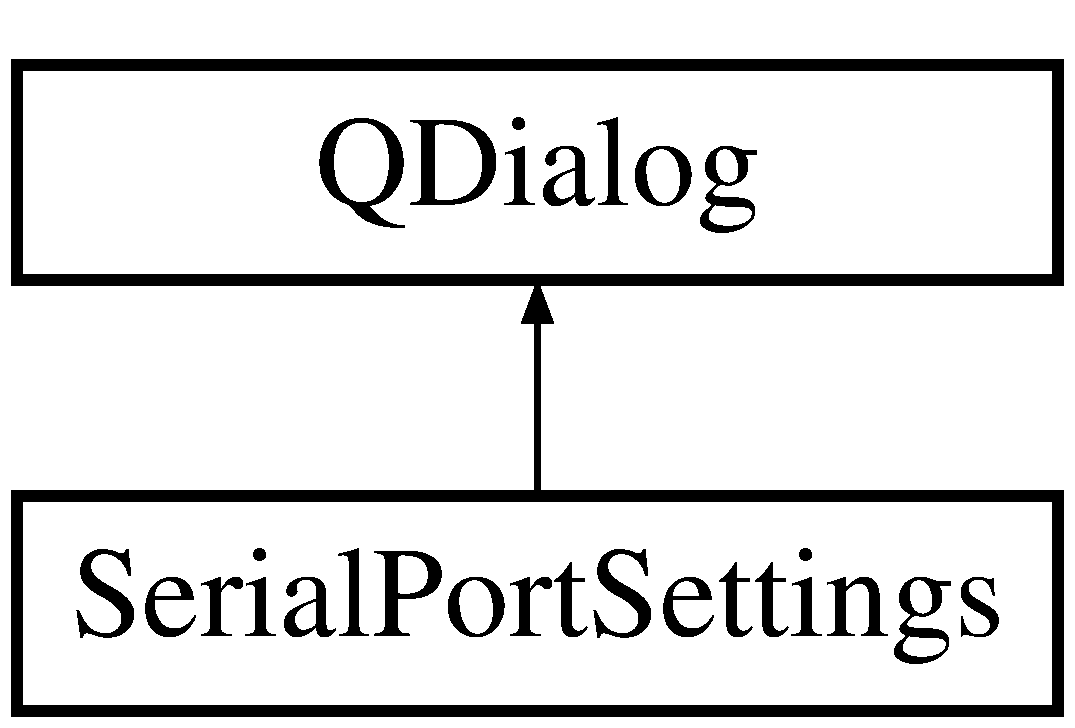
\includegraphics[height=2.000000cm]{class_serial_port_settings}
\end{center}
\end{figure}
\subsection*{Public Member Functions}
\begin{DoxyCompactItemize}
\item 
\hyperlink{class_serial_port_settings_a5563c4a12c42c2487565fb105b9f370c}{Serial\+Port\+Settings} (Q\+Widget $\ast$parent=0)
\item 
\hyperlink{class_serial_port_settings_a4a9fcf3027d619aaef512aeb9f5a2b8f}{$\sim$\+Serial\+Port\+Settings} ()
\item 
Q\+String \hyperlink{class_serial_port_settings_aa1aa401b8b0b394b182bf3e0b8cf146b}{get\+Port} ()
\end{DoxyCompactItemize}
\subsection*{Public Attributes}
\begin{DoxyCompactItemize}
\item 
Q\+String \hyperlink{class_serial_port_settings_ab6d73655f68c506e50fc81b7a595aa3d}{current\+Port}
\end{DoxyCompactItemize}


\subsection{Constructor \& Destructor Documentation}
\mbox{\Hypertarget{class_serial_port_settings_a5563c4a12c42c2487565fb105b9f370c}\label{class_serial_port_settings_a5563c4a12c42c2487565fb105b9f370c}} 
\index{Serial\+Port\+Settings@{Serial\+Port\+Settings}!Serial\+Port\+Settings@{Serial\+Port\+Settings}}
\index{Serial\+Port\+Settings@{Serial\+Port\+Settings}!Serial\+Port\+Settings@{Serial\+Port\+Settings}}
\subsubsection{\texorpdfstring{Serial\+Port\+Settings()}{SerialPortSettings()}}
{\footnotesize\ttfamily Serial\+Port\+Settings\+::\+Serial\+Port\+Settings (\begin{DoxyParamCaption}\item[{Q\+Widget $\ast$}]{parent = {\ttfamily 0} }\end{DoxyParamCaption})\hspace{0.3cm}{\ttfamily [explicit]}}

class for serial communication window \mbox{\Hypertarget{class_serial_port_settings_a4a9fcf3027d619aaef512aeb9f5a2b8f}\label{class_serial_port_settings_a4a9fcf3027d619aaef512aeb9f5a2b8f}} 
\index{Serial\+Port\+Settings@{Serial\+Port\+Settings}!````~Serial\+Port\+Settings@{$\sim$\+Serial\+Port\+Settings}}
\index{````~Serial\+Port\+Settings@{$\sim$\+Serial\+Port\+Settings}!Serial\+Port\+Settings@{Serial\+Port\+Settings}}
\subsubsection{\texorpdfstring{$\sim$\+Serial\+Port\+Settings()}{~SerialPortSettings()}}
{\footnotesize\ttfamily Serial\+Port\+Settings\+::$\sim$\+Serial\+Port\+Settings (\begin{DoxyParamCaption}{ }\end{DoxyParamCaption})}



\subsection{Member Function Documentation}
\mbox{\Hypertarget{class_serial_port_settings_aa1aa401b8b0b394b182bf3e0b8cf146b}\label{class_serial_port_settings_aa1aa401b8b0b394b182bf3e0b8cf146b}} 
\index{Serial\+Port\+Settings@{Serial\+Port\+Settings}!get\+Port@{get\+Port}}
\index{get\+Port@{get\+Port}!Serial\+Port\+Settings@{Serial\+Port\+Settings}}
\subsubsection{\texorpdfstring{get\+Port()}{getPort()}}
{\footnotesize\ttfamily Q\+String Serial\+Port\+Settings\+::get\+Port (\begin{DoxyParamCaption}{ }\end{DoxyParamCaption})}



\subsection{Member Data Documentation}
\mbox{\Hypertarget{class_serial_port_settings_ab6d73655f68c506e50fc81b7a595aa3d}\label{class_serial_port_settings_ab6d73655f68c506e50fc81b7a595aa3d}} 
\index{Serial\+Port\+Settings@{Serial\+Port\+Settings}!current\+Port@{current\+Port}}
\index{current\+Port@{current\+Port}!Serial\+Port\+Settings@{Serial\+Port\+Settings}}
\subsubsection{\texorpdfstring{current\+Port}{currentPort}}
{\footnotesize\ttfamily Q\+String Serial\+Port\+Settings\+::current\+Port}



The documentation for this class was generated from the following files\+:\begin{DoxyCompactItemize}
\item 
C\+:/\+Users/\+Kuba/\+Documents/\+E\+S\+P32tool/\hyperlink{serialportsettings_8h}{serialportsettings.\+h}\item 
C\+:/\+Users/\+Kuba/\+Documents/\+E\+S\+P32tool/\hyperlink{serialportsettings_8cpp}{serialportsettings.\+cpp}\end{DoxyCompactItemize}

\hypertarget{classwifisettings}{}\section{wifisettings Class Reference}
\label{classwifisettings}\index{wifisettings@{wifisettings}}


{\ttfamily \#include $<$wifisettings.\+h$>$}

Inheritance diagram for wifisettings\+:\begin{figure}[H]
\begin{center}
\leavevmode
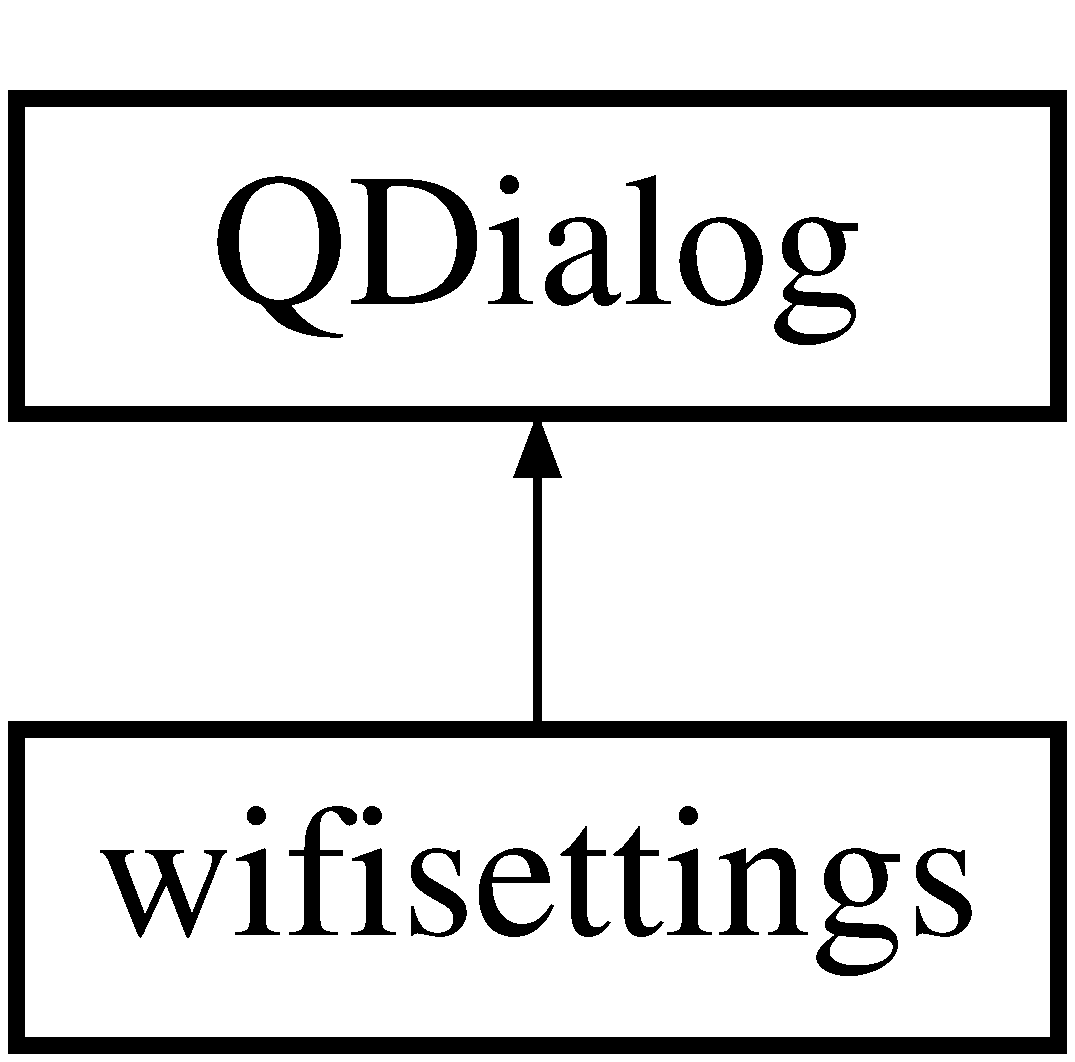
\includegraphics[height=2.000000cm]{classwifisettings}
\end{center}
\end{figure}
\subsection*{Public Member Functions}
\begin{DoxyCompactItemize}
\item 
\hyperlink{classwifisettings_a3ec06d77a62434c5692c40838c1568b0}{wifisettings} (Q\+Widget $\ast$parent=0)
\item 
Q\+String \hyperlink{classwifisettings_a2d5a23c9441438402bf9a858bb742a78}{get\+S\+S\+ID} ()
\item 
Q\+String \hyperlink{classwifisettings_a7ecb69434e89086e1d37158ce8187274}{get\+Password} ()
\item 
Q\+String \hyperlink{classwifisettings_a891601a5caa4148003dcb0d946052b70}{get\+IP} ()
\item 
Q\+String \hyperlink{classwifisettings_a74e1fb264f4b4dfb7d1277d2f895d177}{get\+Port} ()
\item 
\hyperlink{classwifisettings_ae88cdd7ff53ff553f4a8eba0a1dc7aa7}{$\sim$wifisettings} ()
\end{DoxyCompactItemize}


\subsection{Constructor \& Destructor Documentation}
\mbox{\Hypertarget{classwifisettings_a3ec06d77a62434c5692c40838c1568b0}\label{classwifisettings_a3ec06d77a62434c5692c40838c1568b0}} 
\index{wifisettings@{wifisettings}!wifisettings@{wifisettings}}
\index{wifisettings@{wifisettings}!wifisettings@{wifisettings}}
\subsubsection{\texorpdfstring{wifisettings()}{wifisettings()}}
{\footnotesize\ttfamily wifisettings\+::wifisettings (\begin{DoxyParamCaption}\item[{Q\+Widget $\ast$}]{parent = {\ttfamily 0} }\end{DoxyParamCaption})\hspace{0.3cm}{\ttfamily [explicit]}}

class for wifi settings window \mbox{\Hypertarget{classwifisettings_ae88cdd7ff53ff553f4a8eba0a1dc7aa7}\label{classwifisettings_ae88cdd7ff53ff553f4a8eba0a1dc7aa7}} 
\index{wifisettings@{wifisettings}!````~wifisettings@{$\sim$wifisettings}}
\index{````~wifisettings@{$\sim$wifisettings}!wifisettings@{wifisettings}}
\subsubsection{\texorpdfstring{$\sim$wifisettings()}{~wifisettings()}}
{\footnotesize\ttfamily wifisettings\+::$\sim$wifisettings (\begin{DoxyParamCaption}{ }\end{DoxyParamCaption})}



\subsection{Member Function Documentation}
\mbox{\Hypertarget{classwifisettings_a891601a5caa4148003dcb0d946052b70}\label{classwifisettings_a891601a5caa4148003dcb0d946052b70}} 
\index{wifisettings@{wifisettings}!get\+IP@{get\+IP}}
\index{get\+IP@{get\+IP}!wifisettings@{wifisettings}}
\subsubsection{\texorpdfstring{get\+I\+P()}{getIP()}}
{\footnotesize\ttfamily Q\+String wifisettings\+::get\+IP (\begin{DoxyParamCaption}{ }\end{DoxyParamCaption})}

\mbox{\Hypertarget{classwifisettings_a7ecb69434e89086e1d37158ce8187274}\label{classwifisettings_a7ecb69434e89086e1d37158ce8187274}} 
\index{wifisettings@{wifisettings}!get\+Password@{get\+Password}}
\index{get\+Password@{get\+Password}!wifisettings@{wifisettings}}
\subsubsection{\texorpdfstring{get\+Password()}{getPassword()}}
{\footnotesize\ttfamily Q\+String wifisettings\+::get\+Password (\begin{DoxyParamCaption}{ }\end{DoxyParamCaption})}

\mbox{\Hypertarget{classwifisettings_a74e1fb264f4b4dfb7d1277d2f895d177}\label{classwifisettings_a74e1fb264f4b4dfb7d1277d2f895d177}} 
\index{wifisettings@{wifisettings}!get\+Port@{get\+Port}}
\index{get\+Port@{get\+Port}!wifisettings@{wifisettings}}
\subsubsection{\texorpdfstring{get\+Port()}{getPort()}}
{\footnotesize\ttfamily Q\+String wifisettings\+::get\+Port (\begin{DoxyParamCaption}{ }\end{DoxyParamCaption})}

\mbox{\Hypertarget{classwifisettings_a2d5a23c9441438402bf9a858bb742a78}\label{classwifisettings_a2d5a23c9441438402bf9a858bb742a78}} 
\index{wifisettings@{wifisettings}!get\+S\+S\+ID@{get\+S\+S\+ID}}
\index{get\+S\+S\+ID@{get\+S\+S\+ID}!wifisettings@{wifisettings}}
\subsubsection{\texorpdfstring{get\+S\+S\+I\+D()}{getSSID()}}
{\footnotesize\ttfamily Q\+String wifisettings\+::get\+S\+S\+ID (\begin{DoxyParamCaption}{ }\end{DoxyParamCaption})}



The documentation for this class was generated from the following files\+:\begin{DoxyCompactItemize}
\item 
C\+:/\+Users/\+Kuba/\+Documents/\+E\+S\+P32tool/\hyperlink{wifisettings_8h}{wifisettings.\+h}\item 
C\+:/\+Users/\+Kuba/\+Documents/\+E\+S\+P32tool/\hyperlink{wifisettings_8cpp}{wifisettings.\+cpp}\end{DoxyCompactItemize}

\hypertarget{struct_e_s_p32data_1_1_wifi_settings}{}\section{E\+S\+P32data\+:\+:Wifi\+Settings Struct Reference}
\label{struct_e_s_p32data_1_1_wifi_settings}\index{E\+S\+P32data\+::\+Wifi\+Settings@{E\+S\+P32data\+::\+Wifi\+Settings}}


{\ttfamily \#include $<$esp32data.\+h$>$}

\subsection*{Public Attributes}
\begin{DoxyCompactItemize}
\item 
Q\+String \hyperlink{struct_e_s_p32data_1_1_wifi_settings_a59bf3c31c55bea4fa07d0e3d55d5c125}{S\+S\+ID}
\item 
Q\+String \hyperlink{struct_e_s_p32data_1_1_wifi_settings_a38dce639f92290ff219e29d822b4b62c}{wifipassword}
\item 
Q\+String \hyperlink{struct_e_s_p32data_1_1_wifi_settings_acd8a6d52beba9019fba2f7055dee7072}{address\+IP}
\item 
Q\+String \hyperlink{struct_e_s_p32data_1_1_wifi_settings_a32dc462ab6495a371a9916689f6c5bbb}{udpport}
\end{DoxyCompactItemize}


\subsection{Member Data Documentation}
\mbox{\Hypertarget{struct_e_s_p32data_1_1_wifi_settings_acd8a6d52beba9019fba2f7055dee7072}\label{struct_e_s_p32data_1_1_wifi_settings_acd8a6d52beba9019fba2f7055dee7072}} 
\index{E\+S\+P32data\+::\+Wifi\+Settings@{E\+S\+P32data\+::\+Wifi\+Settings}!address\+IP@{address\+IP}}
\index{address\+IP@{address\+IP}!E\+S\+P32data\+::\+Wifi\+Settings@{E\+S\+P32data\+::\+Wifi\+Settings}}
\subsubsection{\texorpdfstring{address\+IP}{addressIP}}
{\footnotesize\ttfamily Q\+String E\+S\+P32data\+::\+Wifi\+Settings\+::address\+IP}

\mbox{\Hypertarget{struct_e_s_p32data_1_1_wifi_settings_a59bf3c31c55bea4fa07d0e3d55d5c125}\label{struct_e_s_p32data_1_1_wifi_settings_a59bf3c31c55bea4fa07d0e3d55d5c125}} 
\index{E\+S\+P32data\+::\+Wifi\+Settings@{E\+S\+P32data\+::\+Wifi\+Settings}!S\+S\+ID@{S\+S\+ID}}
\index{S\+S\+ID@{S\+S\+ID}!E\+S\+P32data\+::\+Wifi\+Settings@{E\+S\+P32data\+::\+Wifi\+Settings}}
\subsubsection{\texorpdfstring{S\+S\+ID}{SSID}}
{\footnotesize\ttfamily Q\+String E\+S\+P32data\+::\+Wifi\+Settings\+::\+S\+S\+ID}

\mbox{\Hypertarget{struct_e_s_p32data_1_1_wifi_settings_a32dc462ab6495a371a9916689f6c5bbb}\label{struct_e_s_p32data_1_1_wifi_settings_a32dc462ab6495a371a9916689f6c5bbb}} 
\index{E\+S\+P32data\+::\+Wifi\+Settings@{E\+S\+P32data\+::\+Wifi\+Settings}!udpport@{udpport}}
\index{udpport@{udpport}!E\+S\+P32data\+::\+Wifi\+Settings@{E\+S\+P32data\+::\+Wifi\+Settings}}
\subsubsection{\texorpdfstring{udpport}{udpport}}
{\footnotesize\ttfamily Q\+String E\+S\+P32data\+::\+Wifi\+Settings\+::udpport}

\mbox{\Hypertarget{struct_e_s_p32data_1_1_wifi_settings_a38dce639f92290ff219e29d822b4b62c}\label{struct_e_s_p32data_1_1_wifi_settings_a38dce639f92290ff219e29d822b4b62c}} 
\index{E\+S\+P32data\+::\+Wifi\+Settings@{E\+S\+P32data\+::\+Wifi\+Settings}!wifipassword@{wifipassword}}
\index{wifipassword@{wifipassword}!E\+S\+P32data\+::\+Wifi\+Settings@{E\+S\+P32data\+::\+Wifi\+Settings}}
\subsubsection{\texorpdfstring{wifipassword}{wifipassword}}
{\footnotesize\ttfamily Q\+String E\+S\+P32data\+::\+Wifi\+Settings\+::wifipassword}



The documentation for this struct was generated from the following file\+:\begin{DoxyCompactItemize}
\item 
C\+:/\+Users/\+Kuba/\+Documents/\+E\+S\+P32tool/\hyperlink{esp32data_8h}{esp32data.\+h}\end{DoxyCompactItemize}

\chapter{File Documentation}
\hypertarget{csvread_8cpp}{}\section{C\+:/\+Users/\+Kuba/\+Documents/\+E\+S\+P32tool/csvread.cpp File Reference}
\label{csvread_8cpp}\index{C\+:/\+Users/\+Kuba/\+Documents/\+E\+S\+P32tool/csvread.\+cpp@{C\+:/\+Users/\+Kuba/\+Documents/\+E\+S\+P32tool/csvread.\+cpp}}
{\ttfamily \#include \char`\"{}csvread.\+h\char`\"{}}\newline
{\ttfamily \#include \char`\"{}ui\+\_\+csvread.\+h\char`\"{}}\newline

\hypertarget{csvread_8h}{}\section{C\+:/\+Users/\+Kuba/\+Documents/\+E\+S\+P32tool/csvread.h File Reference}
\label{csvread_8h}\index{C\+:/\+Users/\+Kuba/\+Documents/\+E\+S\+P32tool/csvread.\+h@{C\+:/\+Users/\+Kuba/\+Documents/\+E\+S\+P32tool/csvread.\+h}}
{\ttfamily \#include $<$Q\+Main\+Window$>$}\newline
{\ttfamily \#include $<$Q\+File$>$}\newline
{\ttfamily \#include $<$Q\+File\+Dialog$>$}\newline
{\ttfamily \#include $<$Q\+Text\+Stream$>$}\newline
{\ttfamily \#include $<$Q\+Debug$>$}\newline
{\ttfamily \#include $<$Q\+String$>$}\newline
{\ttfamily \#include $<$Q\+Standard\+Item\+Model$>$}\newline
\subsection*{Classes}
\begin{DoxyCompactItemize}
\item 
class \hyperlink{class_c_s_vread}{C\+S\+Vread}
\end{DoxyCompactItemize}
\subsection*{Namespaces}
\begin{DoxyCompactItemize}
\item 
 \hyperlink{namespace_ui}{Ui}
\end{DoxyCompactItemize}

\hypertarget{esp32data_8cpp}{}\section{C\+:/\+Users/\+Kuba/\+Documents/\+E\+S\+P32tool/esp32data.cpp File Reference}
\label{esp32data_8cpp}\index{C\+:/\+Users/\+Kuba/\+Documents/\+E\+S\+P32tool/esp32data.\+cpp@{C\+:/\+Users/\+Kuba/\+Documents/\+E\+S\+P32tool/esp32data.\+cpp}}
{\ttfamily \#include \char`\"{}esp32data.\+h\char`\"{}}\newline
{\ttfamily \#include $<$Qt\+Serial\+Port/qserialport.\+h$>$}\newline
{\ttfamily \#include \char`\"{}serialportsettings.\+h\char`\"{}}\newline
{\ttfamily \#include \char`\"{}ui\+\_\+serialportsettings.\+h\char`\"{}}\newline
{\ttfamily \#include \char`\"{}mainwindow.\+h\char`\"{}}\newline
{\ttfamily \#include \char`\"{}Qt\+Serial\+Port/\+Q\+Serial\+Port\char`\"{}}\newline
{\ttfamily \#include \char`\"{}Qt\+Serial\+Port\char`\"{}}\newline
{\ttfamily \#include \char`\"{}Q\+Serial\+Port\char`\"{}}\newline
{\ttfamily \#include $<$Q\+Label$>$}\newline
{\ttfamily \#include $<$Q\+Line\+Edit$>$}\newline
{\ttfamily \#include $<$Q\+Combo\+Box$>$}\newline
{\ttfamily \#include $<$Q\+Spin\+Box$>$}\newline
{\ttfamily \#include $<$Q\+Push\+Button$>$}\newline
{\ttfamily \#include $<$Q\+Grid\+Layout$>$}\newline
{\ttfamily \#include $<$string$>$}\newline
{\ttfamily \#include $<$regex$>$}\newline
{\ttfamily \#include $<$math.\+h$>$}\newline

\hypertarget{esp32data_8h}{}\section{C\+:/\+Users/\+Kuba/\+Documents/\+E\+S\+P32tool/esp32data.h File Reference}
\label{esp32data_8h}\index{C\+:/\+Users/\+Kuba/\+Documents/\+E\+S\+P32tool/esp32data.\+h@{C\+:/\+Users/\+Kuba/\+Documents/\+E\+S\+P32tool/esp32data.\+h}}
{\ttfamily \#include $<$Q\+Object$>$}\newline
{\ttfamily \#include $<$Q\+Serial\+Port$>$}\newline
{\ttfamily \#include $<$Q\+Serial\+Port\+Info$>$}\newline
{\ttfamily \#include \char`\"{}serialportsettings.\+h\char`\"{}}\newline
{\ttfamily \#include \char`\"{}Q\+Timer\char`\"{}}\newline
{\ttfamily \#include $<$Q\+File$>$}\newline
{\ttfamily \#include $<$Q\+Text\+Stream$>$}\newline
{\ttfamily \#include $<$Q\+File\+Dialog$>$}\newline
{\ttfamily \#include $<$Q\+Udp\+Socket$>$}\newline
{\ttfamily \#include $<$Q\+Network\+Datagram$>$}\newline
\subsection*{Classes}
\begin{DoxyCompactItemize}
\item 
class \hyperlink{class_e_s_p32data}{E\+S\+P32data}
\item 
struct \hyperlink{struct_e_s_p32data_1_1_wifi_settings}{E\+S\+P32data\+::\+Wifi\+Settings}
\end{DoxyCompactItemize}

\hypertarget{logger_8cpp}{}\section{C\+:/\+Users/\+Kuba/\+Documents/\+E\+S\+P32tool/logger.cpp File Reference}
\label{logger_8cpp}\index{C\+:/\+Users/\+Kuba/\+Documents/\+E\+S\+P32tool/logger.\+cpp@{C\+:/\+Users/\+Kuba/\+Documents/\+E\+S\+P32tool/logger.\+cpp}}
{\ttfamily \#include \char`\"{}logger.\+h\char`\"{}}\newline

\hypertarget{logger_8h}{}\section{C\+:/\+Users/\+Kuba/\+Documents/\+E\+S\+P32tool/logger.h File Reference}
\label{logger_8h}\index{C\+:/\+Users/\+Kuba/\+Documents/\+E\+S\+P32tool/logger.\+h@{C\+:/\+Users/\+Kuba/\+Documents/\+E\+S\+P32tool/logger.\+h}}
{\ttfamily \#include $<$Q\+String$>$}\newline
{\ttfamily \#include $<$Qfile$>$}\newline
{\ttfamily \#include $<$Q\+Text\+Stream$>$}\newline
{\ttfamily \#include $<$Q\+Time$>$}\newline
{\ttfamily \#include $<$Q\+File\+Dialog$>$}\newline
{\ttfamily \#include $<$Q\+Vector$>$}\newline
\subsection*{Classes}
\begin{DoxyCompactItemize}
\item 
class \hyperlink{classlogger}{logger}
\end{DoxyCompactItemize}

\hypertarget{main_8cpp}{}\section{C\+:/\+Users/\+Kuba/\+Documents/\+E\+S\+P32tool/main.cpp File Reference}
\label{main_8cpp}\index{C\+:/\+Users/\+Kuba/\+Documents/\+E\+S\+P32tool/main.\+cpp@{C\+:/\+Users/\+Kuba/\+Documents/\+E\+S\+P32tool/main.\+cpp}}
{\ttfamily \#include \char`\"{}mainwindow.\+h\char`\"{}}\newline
{\ttfamily \#include $<$Q\+Application$>$}\newline
\subsection*{Functions}
\begin{DoxyCompactItemize}
\item 
int \hyperlink{main_8cpp_a0ddf1224851353fc92bfbff6f499fa97}{main} (int argc, char $\ast$argv\mbox{[}$\,$\mbox{]})
\end{DoxyCompactItemize}


\subsection{Function Documentation}
\mbox{\Hypertarget{main_8cpp_a0ddf1224851353fc92bfbff6f499fa97}\label{main_8cpp_a0ddf1224851353fc92bfbff6f499fa97}} 
\index{main.\+cpp@{main.\+cpp}!main@{main}}
\index{main@{main}!main.\+cpp@{main.\+cpp}}
\subsubsection{\texorpdfstring{main()}{main()}}
{\footnotesize\ttfamily int main (\begin{DoxyParamCaption}\item[{int}]{argc,  }\item[{char $\ast$}]{argv\mbox{[}$\,$\mbox{]} }\end{DoxyParamCaption})}


\hypertarget{mainwindow_8cpp}{}\section{C\+:/\+Users/\+Kuba/\+Documents/\+E\+S\+P32tool/mainwindow.cpp File Reference}
\label{mainwindow_8cpp}\index{C\+:/\+Users/\+Kuba/\+Documents/\+E\+S\+P32tool/mainwindow.\+cpp@{C\+:/\+Users/\+Kuba/\+Documents/\+E\+S\+P32tool/mainwindow.\+cpp}}
{\ttfamily \#include \char`\"{}mainwindow.\+h\char`\"{}}\newline
{\ttfamily \#include \char`\"{}ui\+\_\+mainwindow.\+h\char`\"{}}\newline
{\ttfamily \#include \char`\"{}serialportsettings.\+h\char`\"{}}\newline
{\ttfamily \#include \char`\"{}esp32data.\+h\char`\"{}}\newline
{\ttfamily \#include $<$Q\+Label$>$}\newline
{\ttfamily \#include $<$Q\+Line\+Edit$>$}\newline
{\ttfamily \#include $<$Q\+Combo\+Box$>$}\newline
{\ttfamily \#include $<$Q\+Spin\+Box$>$}\newline
{\ttfamily \#include $<$Q\+Push\+Button$>$}\newline
{\ttfamily \#include $<$Q\+Grid\+Layout$>$}\newline
{\ttfamily \#include $<$Qt\+Serial\+Port/\+Q\+Serial\+Port\+Info$>$}\newline
{\ttfamily \#include $<$Q\+Debug$>$}\newline
{\ttfamily \#include $<$Qfile$>$}\newline
{\ttfamily \#include $<$Q\+Text\+Stream$>$}\newline
{\ttfamily \#include $<$Q\+Time$>$}\newline
{\ttfamily \#include $<$Q\+File\+Dialog$>$}\newline
{\ttfamily \#include \char`\"{}logger.\+h\char`\"{}}\newline
{\ttfamily \#include $<$wifisettings.\+h$>$}\newline

\hypertarget{mainwindow_8h}{}\section{C\+:/\+Users/\+Kuba/\+Documents/\+E\+S\+P32tool/mainwindow.h File Reference}
\label{mainwindow_8h}\index{C\+:/\+Users/\+Kuba/\+Documents/\+E\+S\+P32tool/mainwindow.\+h@{C\+:/\+Users/\+Kuba/\+Documents/\+E\+S\+P32tool/mainwindow.\+h}}
{\ttfamily \#include $<$Q\+Main\+Window$>$}\newline
{\ttfamily \#include \char`\"{}esp32data.\+h\char`\"{}}\newline
{\ttfamily \#include \char`\"{}csvread.\+h\char`\"{}}\newline
{\ttfamily \#include \char`\"{}logger.\+h\char`\"{}}\newline
{\ttfamily \#include $<$Q\+Elapsed\+Timer$>$}\newline
\subsection*{Classes}
\begin{DoxyCompactItemize}
\item 
class \hyperlink{class_main_window}{Main\+Window}
\end{DoxyCompactItemize}
\subsection*{Namespaces}
\begin{DoxyCompactItemize}
\item 
 \hyperlink{namespace_ui}{Ui}
\end{DoxyCompactItemize}

\hypertarget{serialportsettings_8cpp}{}\section{C\+:/\+Users/\+Kuba/\+Documents/\+E\+S\+P32tool/serialportsettings.cpp File Reference}
\label{serialportsettings_8cpp}\index{C\+:/\+Users/\+Kuba/\+Documents/\+E\+S\+P32tool/serialportsettings.\+cpp@{C\+:/\+Users/\+Kuba/\+Documents/\+E\+S\+P32tool/serialportsettings.\+cpp}}
{\ttfamily \#include \char`\"{}serialportsettings.\+h\char`\"{}}\newline
{\ttfamily \#include \char`\"{}ui\+\_\+serialportsettings.\+h\char`\"{}}\newline
{\ttfamily \#include \char`\"{}esp32data.\+h\char`\"{}}\newline
{\ttfamily \#include \char`\"{}mainwindow.\+h\char`\"{}}\newline
{\ttfamily \#include \char`\"{}Qt\+Serial\+Port/\+Q\+Serial\+Port\char`\"{}}\newline
{\ttfamily \#include \char`\"{}Qt\+Serial\+Port\char`\"{}}\newline
{\ttfamily \#include \char`\"{}Q\+Serial\+Port\char`\"{}}\newline
{\ttfamily \#include $<$Q\+Label$>$}\newline
{\ttfamily \#include $<$Q\+Line\+Edit$>$}\newline
{\ttfamily \#include $<$Q\+Combo\+Box$>$}\newline
{\ttfamily \#include $<$Q\+Spin\+Box$>$}\newline
{\ttfamily \#include $<$Q\+Push\+Button$>$}\newline
{\ttfamily \#include $<$Q\+Grid\+Layout$>$}\newline

\hypertarget{serialportsettings_8h}{}\section{C\+:/\+Users/\+Kuba/\+Documents/\+E\+S\+P32tool/serialportsettings.h File Reference}
\label{serialportsettings_8h}\index{C\+:/\+Users/\+Kuba/\+Documents/\+E\+S\+P32tool/serialportsettings.\+h@{C\+:/\+Users/\+Kuba/\+Documents/\+E\+S\+P32tool/serialportsettings.\+h}}
{\ttfamily \#include $<$Q\+Dialog$>$}\newline
{\ttfamily \#include \char`\"{}esp32data.\+h\char`\"{}}\newline
\subsection*{Classes}
\begin{DoxyCompactItemize}
\item 
class \hyperlink{class_serial_port_settings}{Serial\+Port\+Settings}
\end{DoxyCompactItemize}
\subsection*{Namespaces}
\begin{DoxyCompactItemize}
\item 
 \hyperlink{namespace_ui}{Ui}
\end{DoxyCompactItemize}

\hypertarget{wifisettings_8cpp}{}\section{C\+:/\+Users/\+Kuba/\+Documents/\+E\+S\+P32tool/wifisettings.cpp File Reference}
\label{wifisettings_8cpp}\index{C\+:/\+Users/\+Kuba/\+Documents/\+E\+S\+P32tool/wifisettings.\+cpp@{C\+:/\+Users/\+Kuba/\+Documents/\+E\+S\+P32tool/wifisettings.\+cpp}}
{\ttfamily \#include \char`\"{}wifisettings.\+h\char`\"{}}\newline
{\ttfamily \#include \char`\"{}ui\+\_\+wifisettings.\+h\char`\"{}}\newline
{\ttfamily \#include $<$esp32data.\+h$>$}\newline
{\ttfamily \#include $<$mainwindow.\+h$>$}\newline

\hypertarget{wifisettings_8h}{}\section{C\+:/\+Users/\+Kuba/\+Documents/\+E\+S\+P32tool/wifisettings.h File Reference}
\label{wifisettings_8h}\index{C\+:/\+Users/\+Kuba/\+Documents/\+E\+S\+P32tool/wifisettings.\+h@{C\+:/\+Users/\+Kuba/\+Documents/\+E\+S\+P32tool/wifisettings.\+h}}
{\ttfamily \#include $<$Q\+Dialog$>$}\newline
\subsection*{Classes}
\begin{DoxyCompactItemize}
\item 
class \hyperlink{classwifisettings}{wifisettings}
\end{DoxyCompactItemize}
\subsection*{Namespaces}
\begin{DoxyCompactItemize}
\item 
 \hyperlink{namespace_ui}{Ui}
\end{DoxyCompactItemize}

%--- End generated contents ---

% Index
\backmatter
\newpage
\phantomsection
\clearemptydoublepage
\addcontentsline{toc}{chapter}{Index}
\printindex

\end{document}
